\chapter{Metodología}\label{cap3} % con la palabra capitulo
%\addcontentsline{toc}{chapter}{Capítulo 2: Marco Teórico} % si queremos que aparezca en el Í­ndice
%\markboth{Capítulo 2: Marco Teórico}{Capítulo 2: Marco Teórico} % encabezado
\graphicspath{./imagenes}
En la Figura \ref{fig:ejem1} se muestra una imagen de ejemplo 
\begin{figure}[hbtp]
\centering
\includegraphics[scale=0.1]{imagenes/tomas.jpg}
\caption{Photo by Tomáš Malík on \href{https://unsplash.com/}{Unsplash}}
\label{fig:ejem1}
\end{figure}
\clearpage
En la Figura \ref{fig:ejem:2} se muestra un ejemplo de multiples figuras en una sola.
\begin{figure}[hbtp]
\centering
\subfigure[Photo by dylan nolte on \href{https://unsplash.com/}{Unsplash}]{\includegraphics[scale=0.03]{imagenes/dylan.jpg}}
\subfigure[Photo by Kai Dahms on \href{https://unsplash.com/}{Unsplash}]{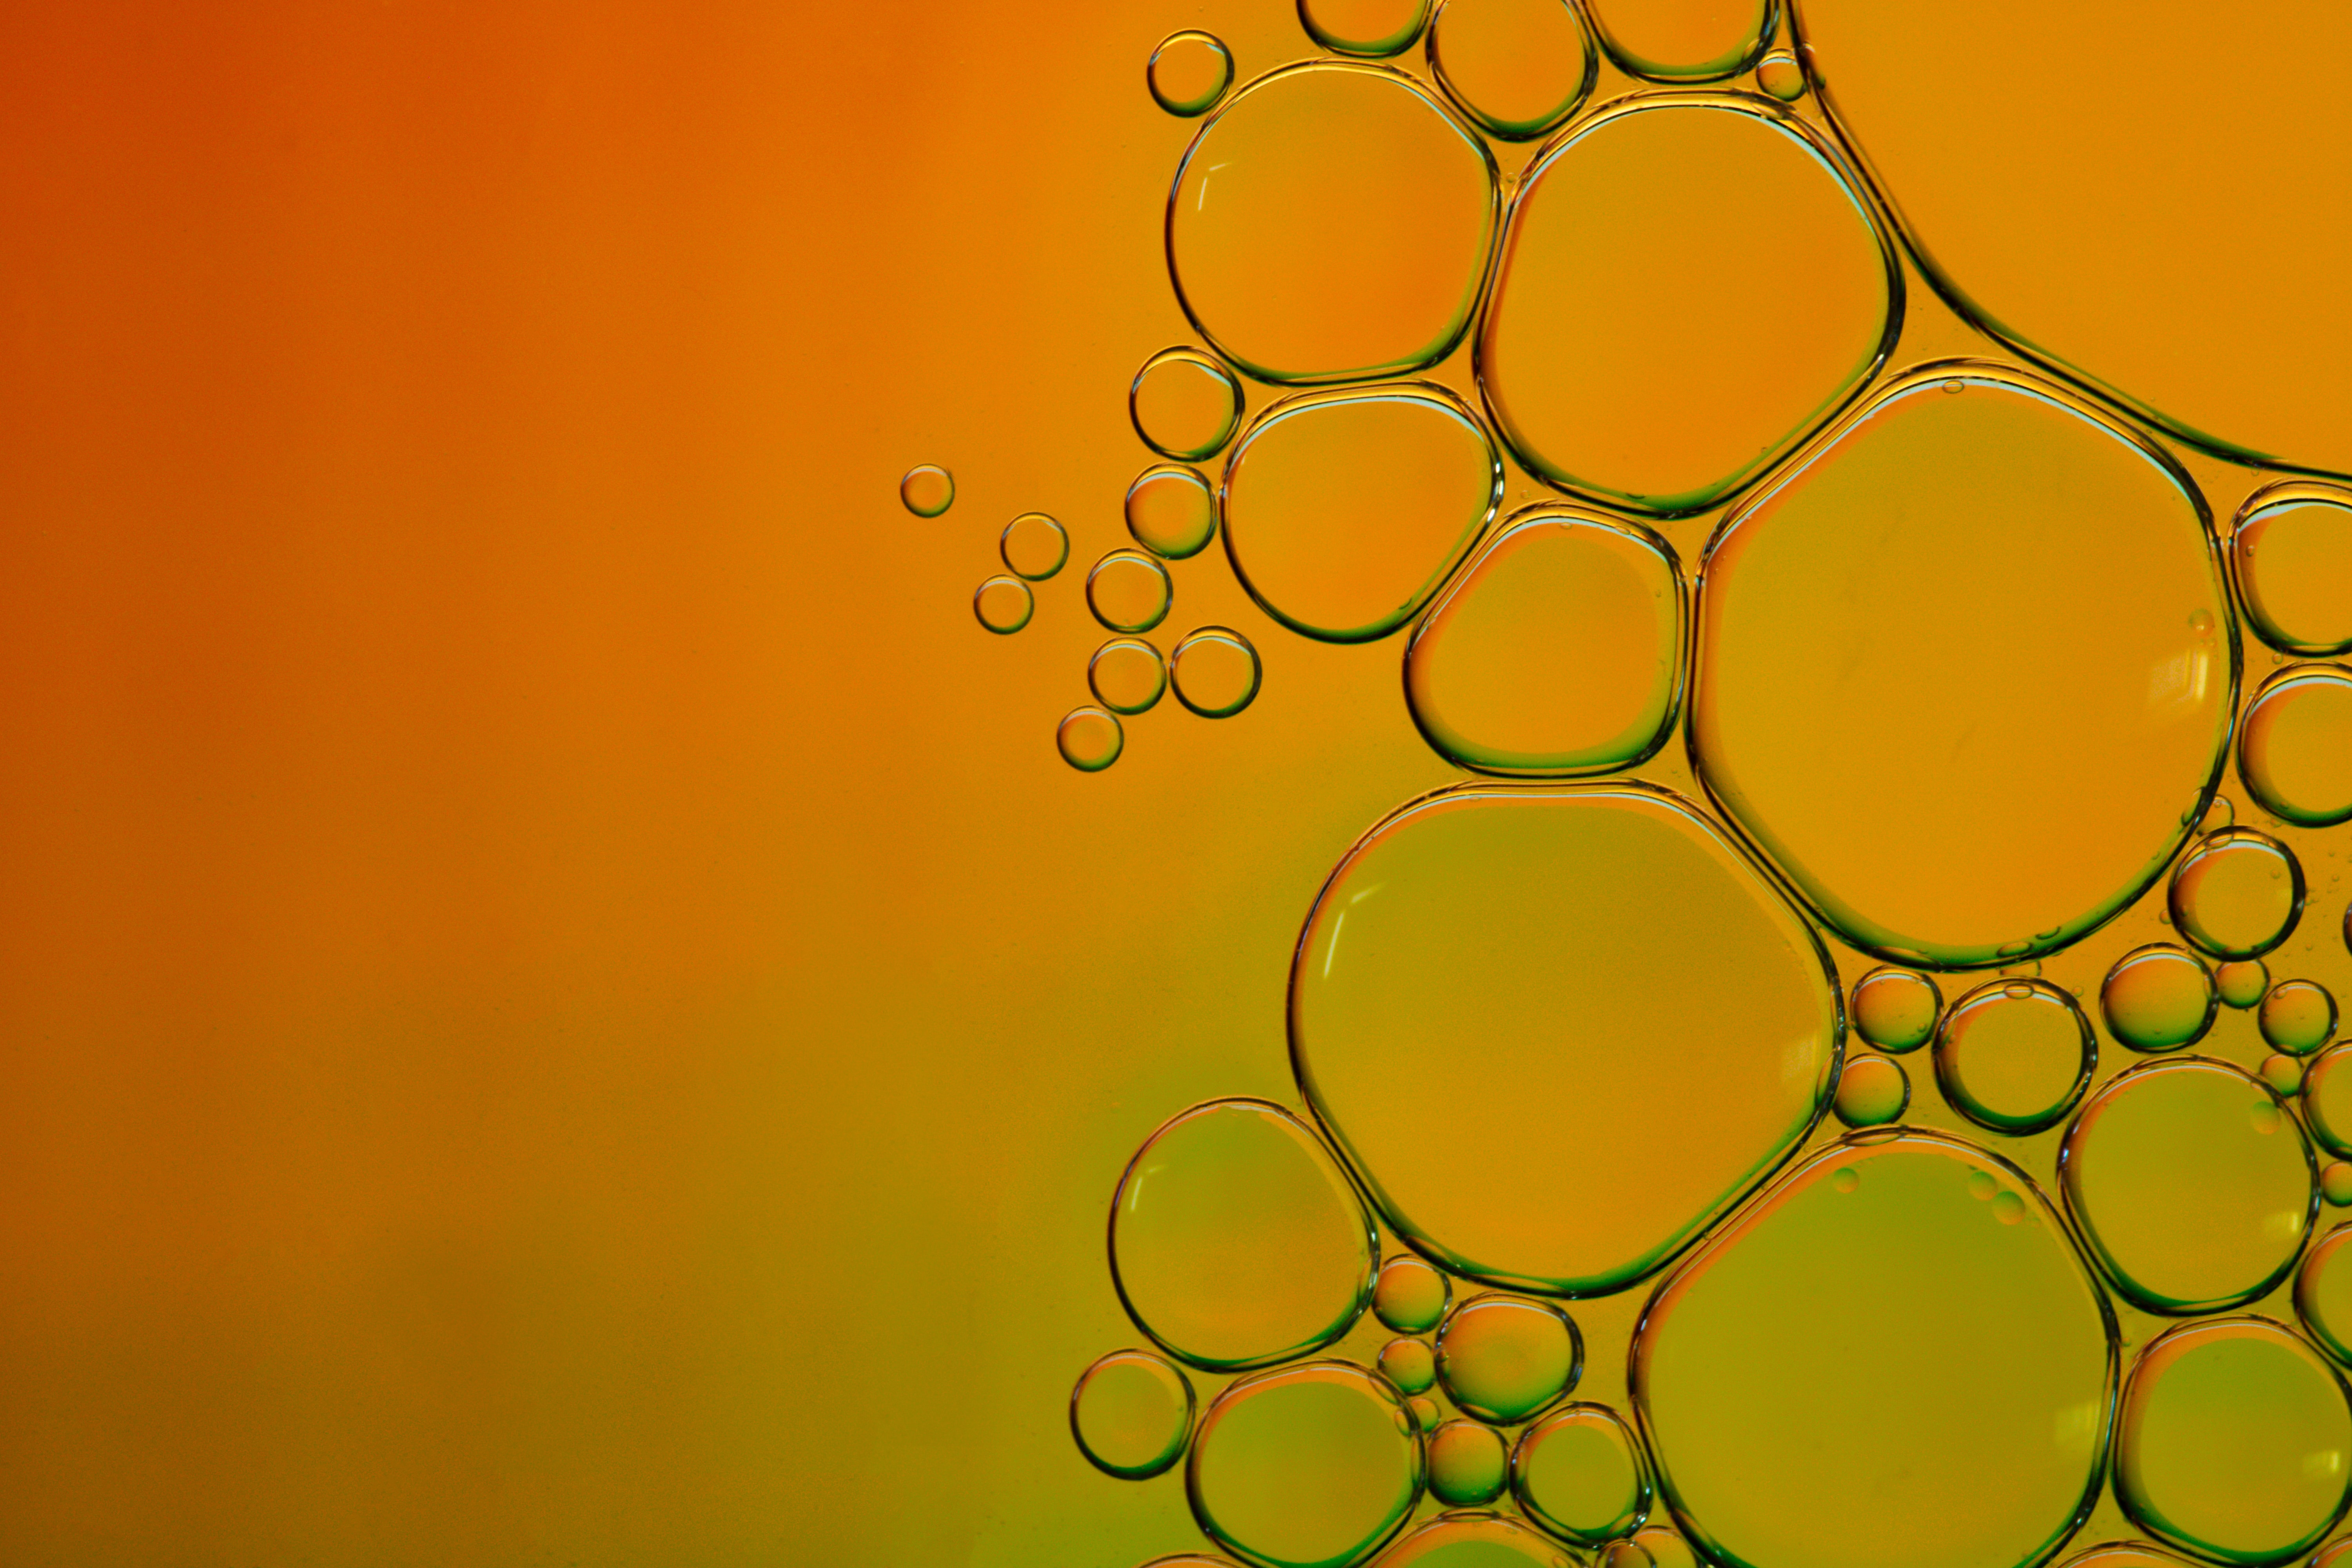
\includegraphics[scale=0.03]{imagenes/kai.jpg}}\\
\subfigure[Photo by Raul Angel on \href{https://unsplash.com/}{Unsplash}]{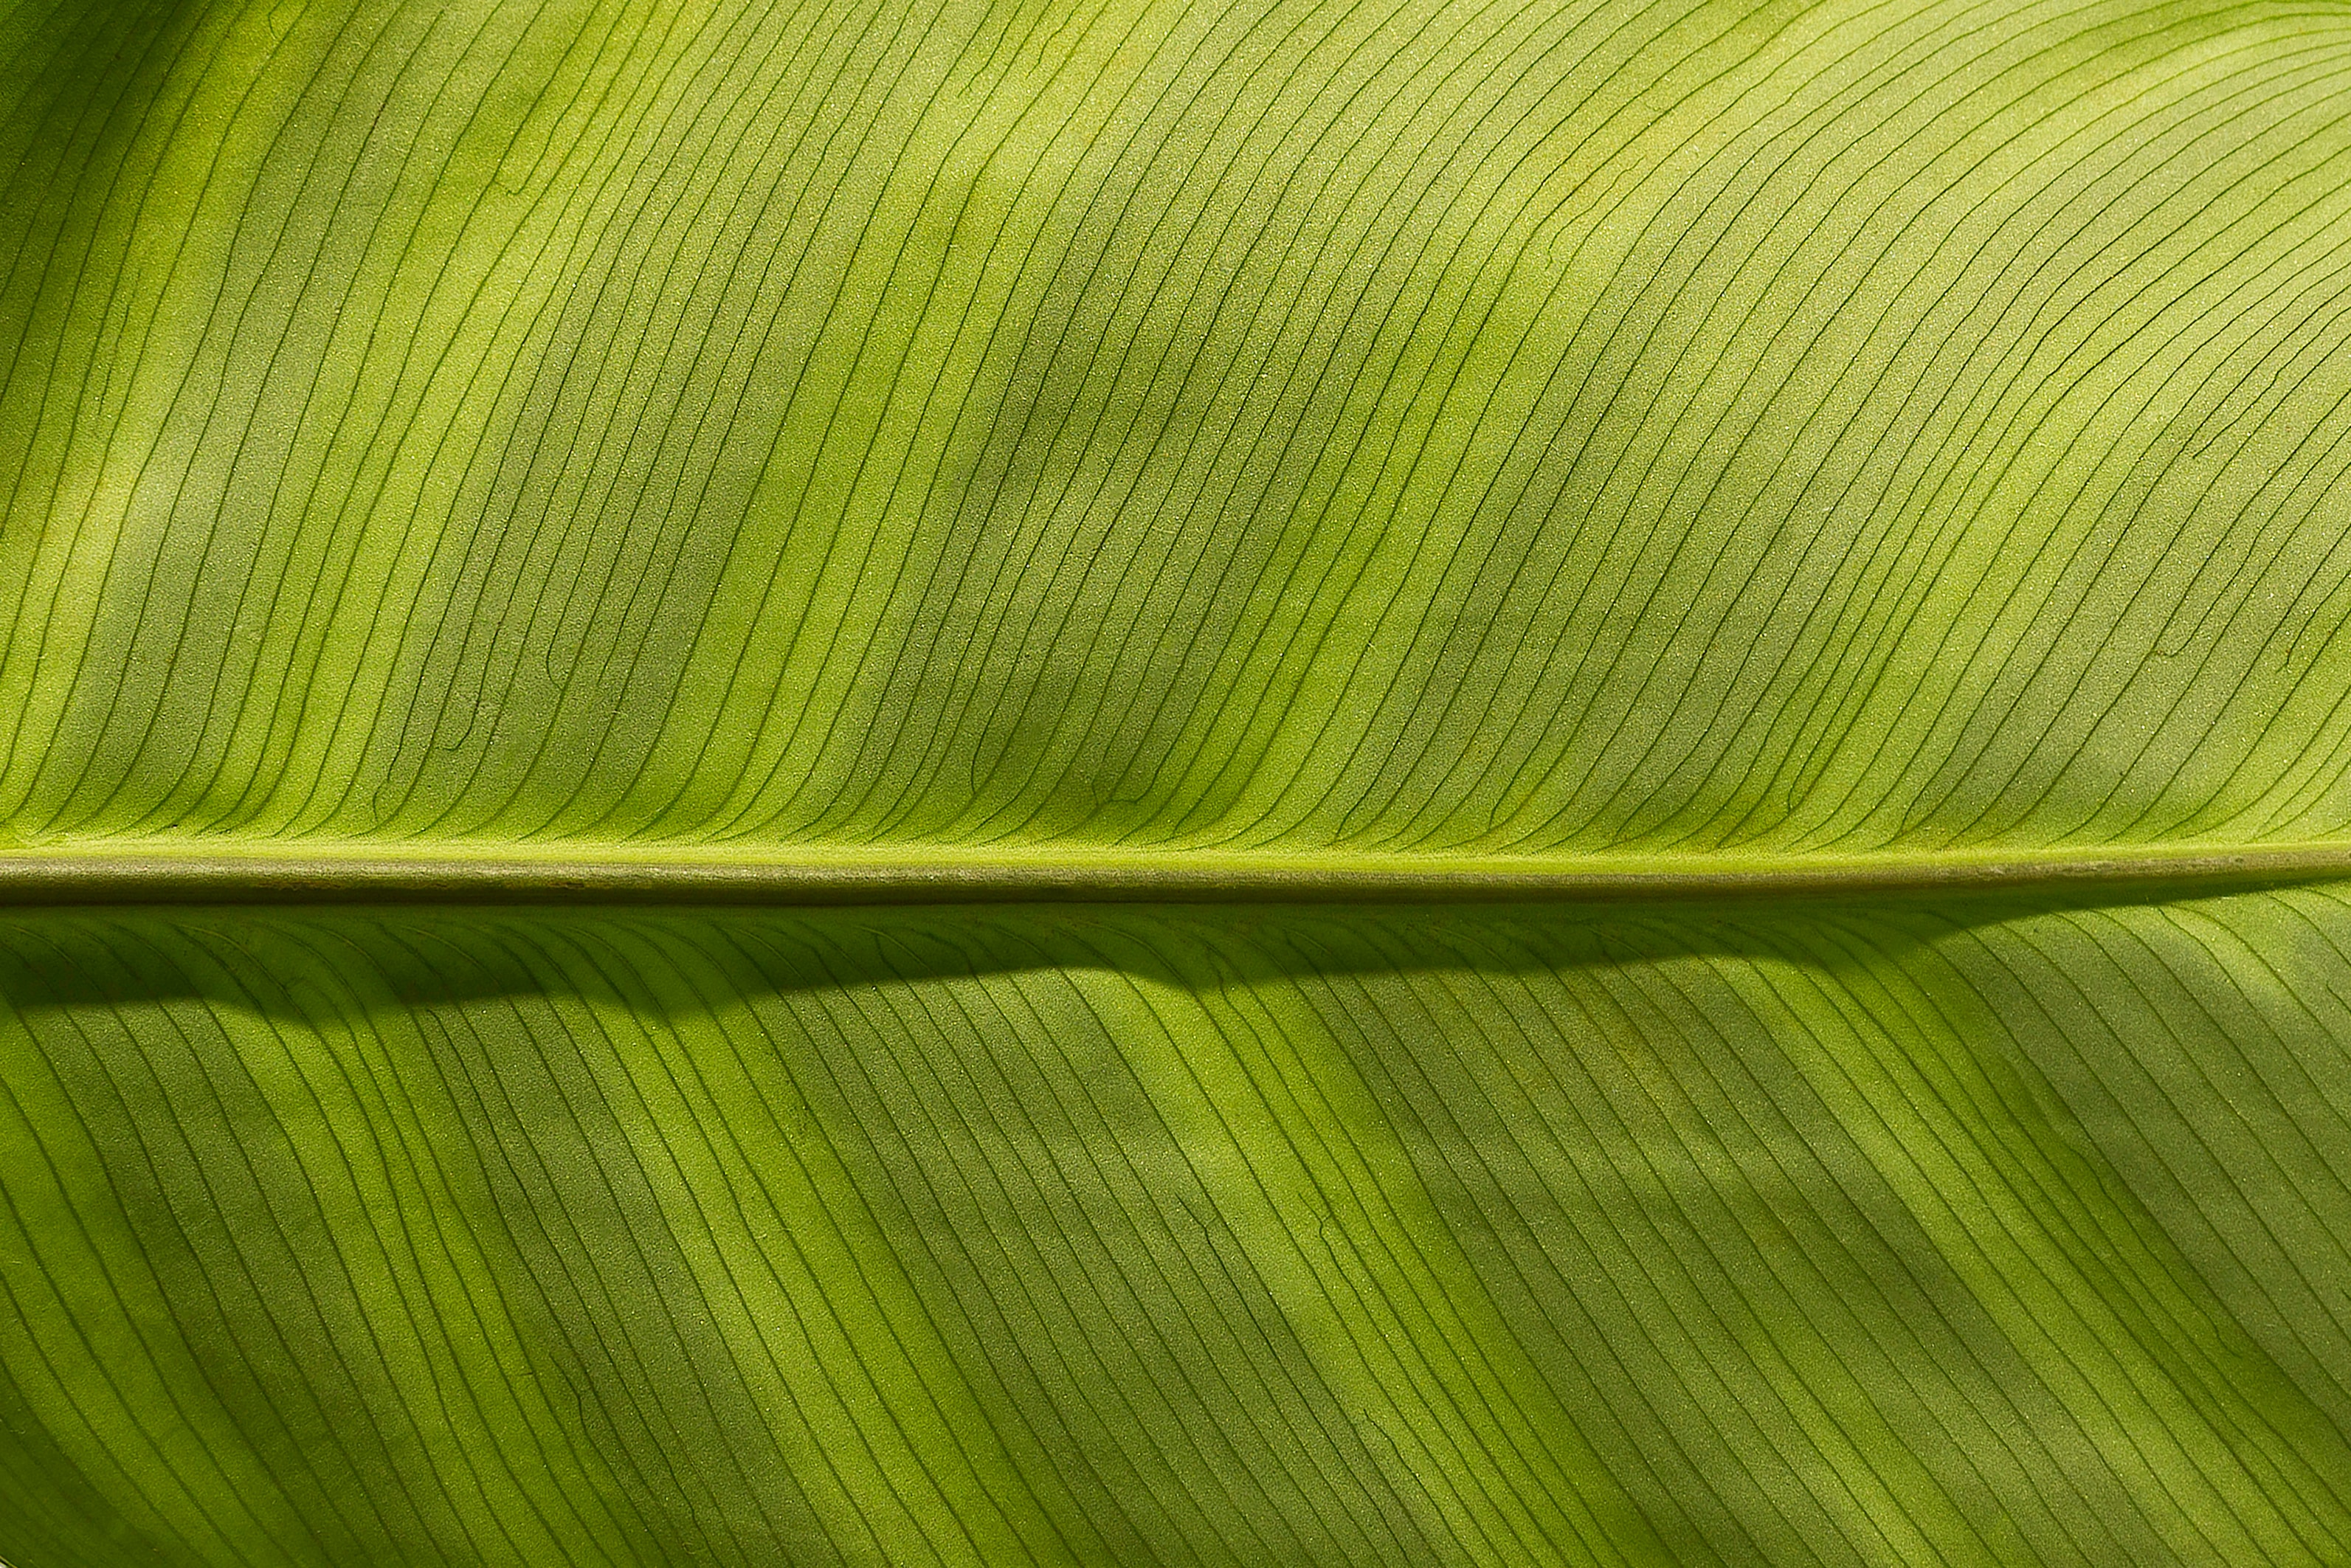
\includegraphics[scale=0.056]{imagenes/raul.jpg}}
\subfigure[Photo by Stéphane Mingot on \href{https://unsplash.com/}{Unsplash}]{\includegraphics[scale=0.04]{imagenes/stephane.jpg}}\\
\caption{Ejemplo de ambiente Figure con múltiples imágenes}
\label{fig:ejem:2}
\end{figure}

La Tabla \ref{tab:ejem1} es un ejemplo para el estudiante sobre como construir tablas

\begin{table}[h]
\caption{Ejemplo de tabla.}
\begin{center}
\begin{tabular}{ cccc } 
\hline
col1 & col2 & col3 \\
\hline
\multirow{3}{4em}{Multiple row} & cell2 & cell3 \\ 
& cell5 & cell6 \\ 
& cell8 & cell9 \\ 
\hline
\end{tabular}
\label{tab:ejem1}
\end{center}
\end{table}


\clearpage%